\documentclass[a4paper]{report}
\usepackage{graphicx} % Required for inserting images

\usepackage[portuguese]{babel}
\usepackage{a4wide}
\pagenumbering{arabic}

\usepackage{graphicx}
\usepackage{hyperref}
\usepackage{listings}
\usepackage{indentfirst}
\usepackage{float}
\usepackage{outlines}
\usepackage{subfigure}

\setlength{\parskip}{1em}
\renewcommand\thesection{\arabic{section}}

\pagenumbering{arabic}
\usepackage{fancyhdr}
\usepackage{lastpage}
\pagestyle{fancy}
\fancyhf{}
\rfoot{Page \thepage \hspace{1pt} of \pageref{LastPage}}

\title{Processamento de Linguagens}

\author{João Silva (A91671)
        \and Luís Vilas (A91697)
        \and Paula Marques (A90088)}
\date{Ano Letivo 2022/2023}

\begin{document}

\begin{minipage}{0.9\linewidth}
    \begin{center}
        \centering
        
\includegraphics[width=0.8\textwidth]{imagens/uminho.png}\par\vspace{1cm}
        \href{https://www.uminho.pt/PT}
        {\scshape\LARGE Universidade do Minho} \par
        \vspace{0.6cm}
        \href{https://www.uminho.pt/PT/ensino/oferta-educativa/Cursos-Conferentes-a-Grau/_layouts/15/UMinho.PortalUM.UI/Pages/CatalogoCursoDetail.aspx?itemId=4079&catId=12}
        {\scshape\Large Licenciatura em Engenharia Informática} \par
        \vspace{1.3cm}
        \textbf{Grupo 12}
        \vspace{0.6cm}
    %		\href{https://github.com/zemmartins/Projeto-DSS}{\textbf{GitHub do Projeto}} \par
        \maketitle
        \begin{figure}[H]
            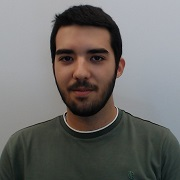
\includegraphics[width=0.31\linewidth]{imagens/Aluno1.jpg}
            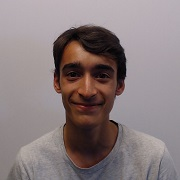
\includegraphics[width=0.31\linewidth]{imagens/Aluno2.png}
            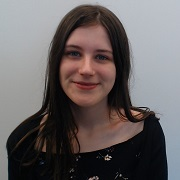
\includegraphics[width=0.31\linewidth]{imagens/Aluno3.jpg}
        \end{figure}
    \end{center}
\end{minipage}


\renewcommand{\contentsname}{Índice}
\tableofcontents

\newpage


\section{Introdução}
\paragraph{}
No âmbito da Unidade Curricular de Processamento de Linguagens, foi-nos pedida a realização de um \textit{Parser}, utilizando as técnicas cultivadas ao longo do semestre, como é o caso do \textit{YACC, Lexer, Python}.
\paragraph{}
Tal como o ser humano, os computadors também têm capacidade de fazer a análise sintática de texto. Realizam esta operação através da decomposição da informação de entrada em unidades estruturais, tais como arrays ou mesmo dicionários. A esta transformação, chamamos de \textit{parsing} e este é composto por \textit{tokens}. 
\paragraph{}
Na realização deste projecto prático utilizamos a linguagem de programação Python, bem como alguns módulos do mesmo, para conseguirmos analisar um ficheiro escrito em \textit{TOML} e convertê-lo para \textit{JSON}, que é um formato compacto e amplamente usado para trocar informação, bem como transferencia entre \textit{API} e clientes.
\newpage

\section{Enunciado}
\paragraph{} Para iniciar, começamos por escolher  o enunciado estaria mais adaptado aquilo que pretendiamos. Escolhemos então o \textit{2.6 2.6 Conversor toml-json }, tal como podemos ver no enunciado apresentado pelos docentes:
\begin{figure}[H]
    \centering
    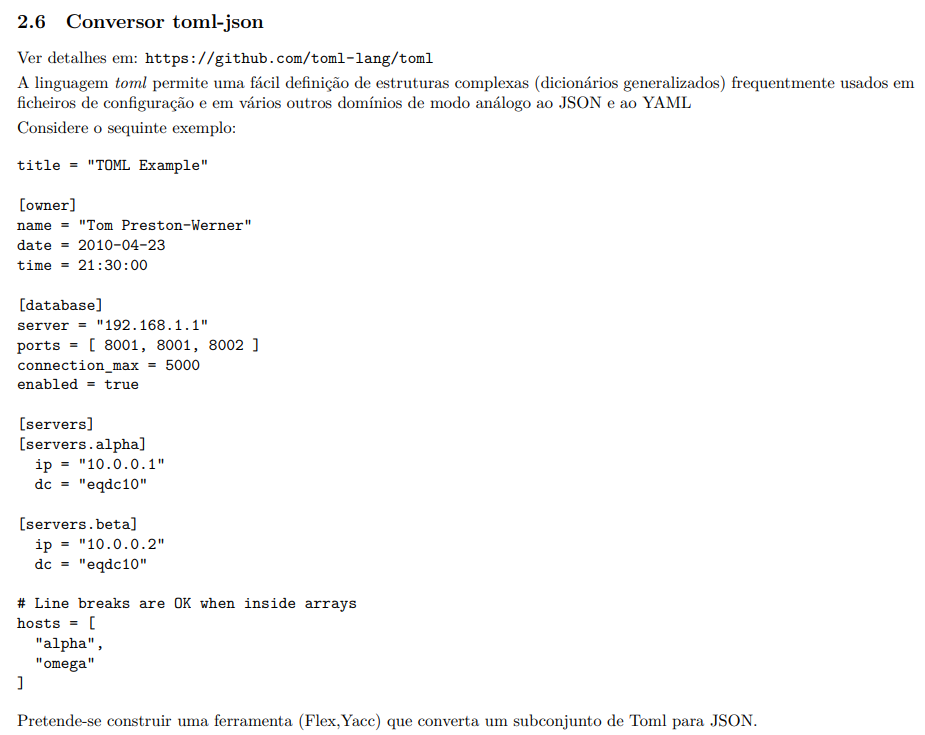
\includegraphics[width = \textwidth]{imagens/TrabalhosProposto.png}
    \caption{Trabalho escolhido pelo grupo}
    \label{fig:my_label}
\end{figure}

\newpage

\section{Linguagem Original \textit{TOML}}
\paragraph{} O TOML é uma linguagem de programação que foi desenvolvida para ser uma linguagem minimalista para a criação de ficheiros de configuração. Também tem o objetivo de ser de fácil leitura e, inversamente, de fácill escrita. 
\subsection{Estrutura da Linguagem}
\begin{figure}[H]
    \centering
    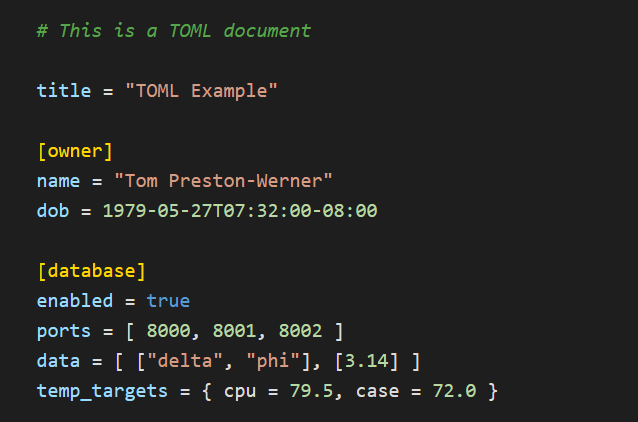
\includegraphics{imagens/ExemploTOML.png}
    \caption{Exemplo de ficheiro \textit{TOML}}
    \label{fig:my_label}
\end{figure}
\paragraph{} Tal como podemos ver na Figura acima, o ficheiro é facilmente legível por qualquer pessoa, mesmo sem qualquer conhecimento da linguagem de programação.

\subsection{Declarações}
As declarações de variavéis são feitas de forma similar a outras linguagens. Embora estas não contenham um \textit{";"} no final.
Abaixo podemos ver mais alguns exemplos de declarações de variáveis, no TOML:
\paragraph{}
title = "Exemplo"
\paragraph{}
livros = ["Maias", "Lusíadas]
\paragraph{}
servidor = { memoria = 16, cores = 4 }
\paragraph{}
[servidor]
cores = 4
memoria = 16
\paragraph{}
Através deste exemplo é possível interpretar que existem diversas formas de definir diferentes tipos de variáveis, compostas por vezes por elementos dentro da mesma "table", ou seja, um dicionário em \textit{Python}

\subsection{Input e Output}
No inicio da execução do programa, é solicitado ao utilizador para introduzir o nome do ficheiro \textit{TOML} a ser interpretado, para ser convertido para \textit{JSON}, tal como podemos ver na Figura abaixo.
\begin{figure}[H]
    \centering
    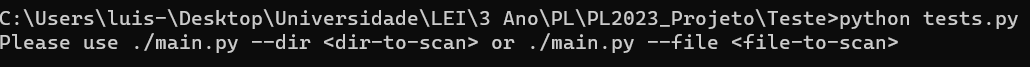
\includegraphics[scale=0.7]{imagens/ExecucaoRequirements.png}
    \caption{Exemplo de execução \textit{TOML}}
    \label{fig:my_label}
\end{figure}


\paragraph{}
Nesse sentido, após ser todo interpretado, o programa escreve no terminal o \textit{JSON} correspondente à interpretação e conversão. Além de ser escrito no terminal, também é escrito num ficheiro de output, para ficar guardado no disco do utilizador, como podemos ver na Figura que se segue:

\begin{figure}[H]
    \centering
    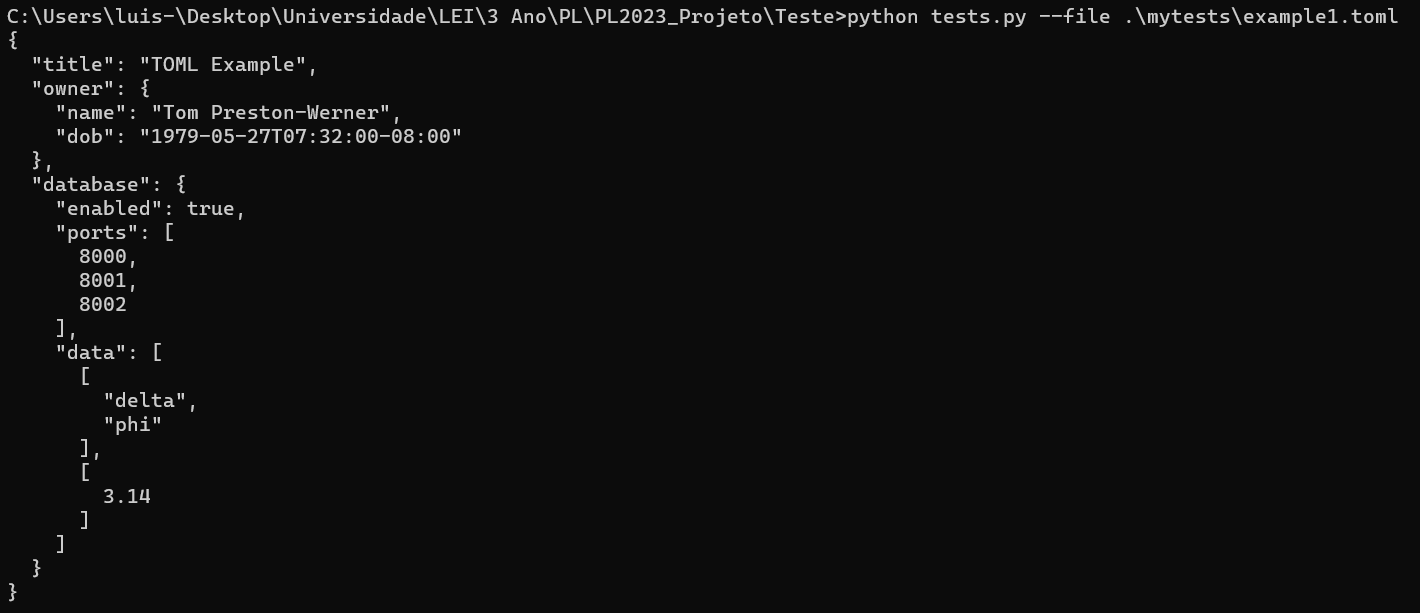
\includegraphics[scale=0.4]{imagens/ExemploParsed.png}
    \caption{Exemplo de parse de um ficheiro \textit{TOML}}
    \label{fig:my_label}
\end{figure}

\newpage

\section{Regras de Tradução}
Em Python, um token de compilação é uma unidade léxica, ou seja, um elemento básico de sintaxe que compõe um programa em Python. Os tokens são as peças individuais que formam o código-fonte Python.
\begin{figure}[H]
    \centering
    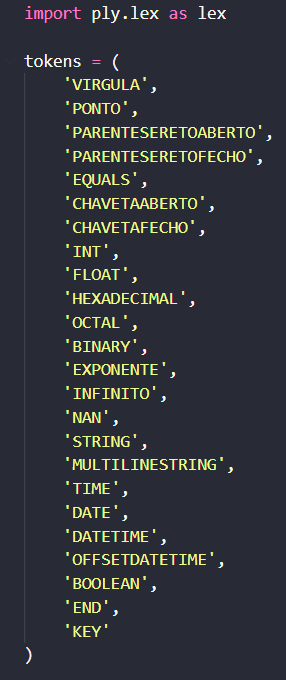
\includegraphics[scale=0.4]{imagens/pt.png}
    \caption{Tokens}
    \label{fig:my_label}
\end{figure}
\begin{figure}[H]
    \centering
    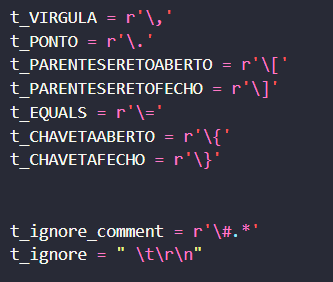
\includegraphics[scale=0.4]{imagens/image.png}
    \caption{Tokens}
    \label{fig:my_label}
\end{figure}
\begin{figure}[H]
    \centering
    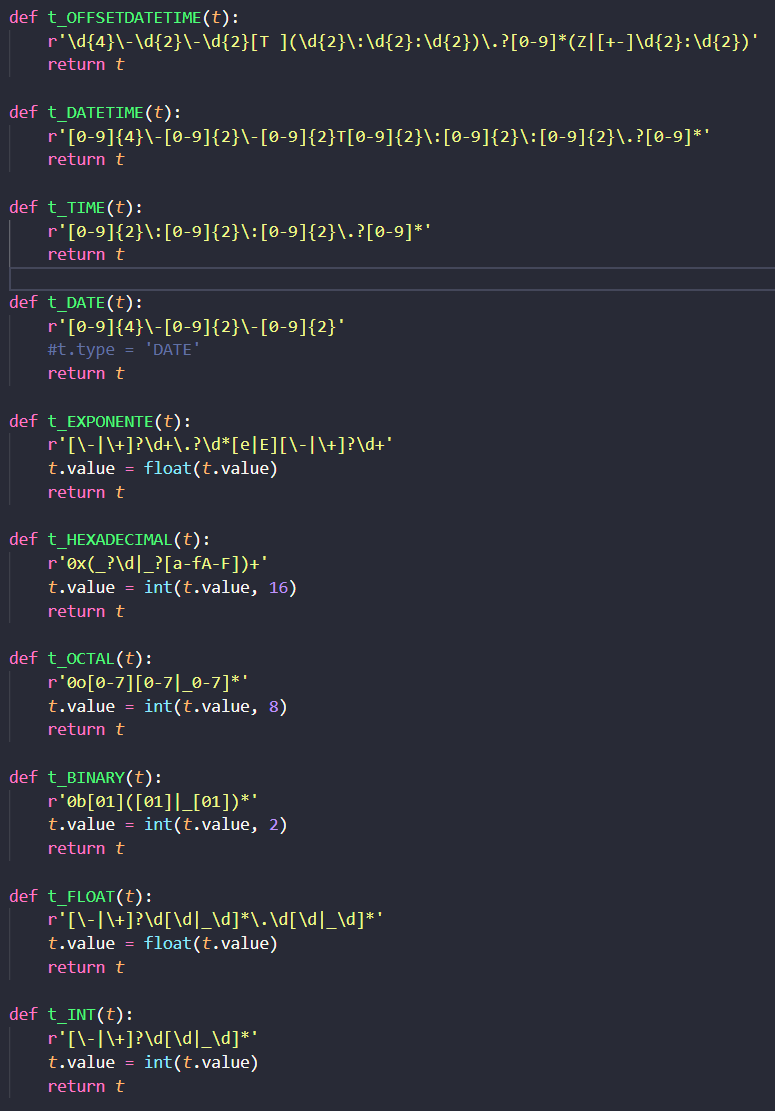
\includegraphics[scale=0.4]{imagens/l.png}
    \caption{Tokens}
    \label{fig:my_label}
\end{figure}
\begin{figure}[H]
    \centering
    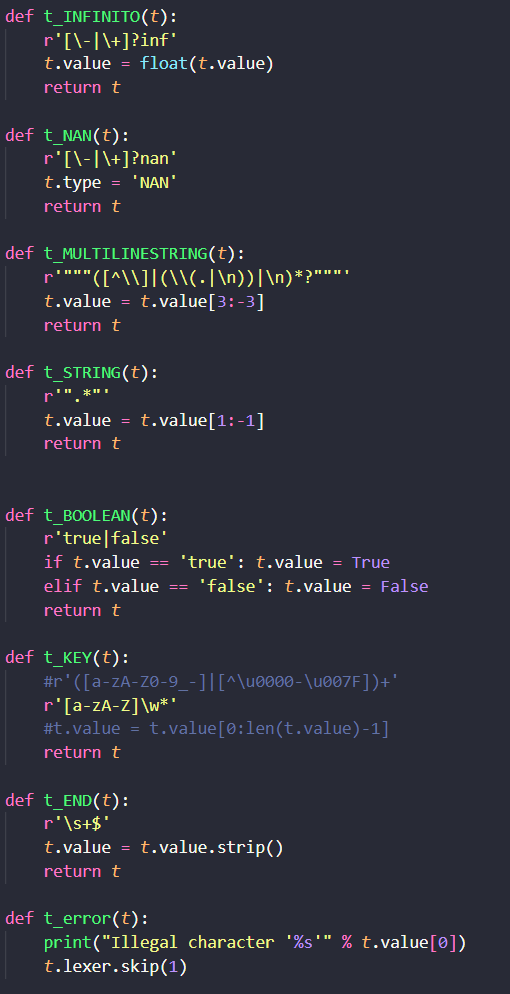
\includegraphics[scale=0.4]{imagens/llll.png}
    \caption{Tokens}
    \label{fig:my_label}
\end{figure}
\paragraph{}
O Yacc permite definir uma gramática formal usando uma notação especializada chamada gramática BNF (Backus-Naur Form). Essa gramática descreve a estrutura sintática da linguagem a ser analisada. Com base na gramática fornecida, o Yacc gera um analisador sintático que pode analisar um programa escrito nessa linguagem e identificar sua estrutura gramatical.
\paragraph{}






\newpage
\section{Conclusão}
Este projeto permitiu-nos aprofundar os conhecimentos adquiridos nas aulas de Processamento de Linguagens e, dessa forma, ter uma ideia de como fnuncionam os compiladores, tais como o gcc, que converte para código máquina código escrito em C. 
\paragraph{}
Gostaríamos de ter conseguido criar um CLiente/Servidor que permitisse implementar a ferramenta desenvolvida, para poder se acessivel mais facilmente, mas tal não foi possível, tendo em conto o tempo que estava destinado à realização deste projeto. Embora essas nossas expectativas, fizemos tudo aquilo que era requesitado pelo enunciado publicado e, dessa forma estamos satisfeitos com o trabalho realzado.

\end{document}
